% called by main.tex
%
\chapter{Correlation between GDP and expected lifespan}
\label{part3}
In this part, an exploration will be undertaken to discern whether there exists a correlation between a country's economic affluence and the life expectancy of its populace. Employing linear regression as a statistical tool to examine the potential relationship between these two variables is deemed appropriate for obtaining insights into this inquiry.

First we'll be listing the formula should be used for the calculation.

The correlation coefficient $\rho$ between 2 fields can be \underline{estimated} using this formula:
\begin{center}
  {\fontsize{20}{20}\selectfont
    \( r = \frac{n \sum{xy} - \sum{x} \sum{y}}{\sqrt{n \sum{x^2} - ({\sum{x}})^2} \sqrt{n \sum{y^2}- ({\sum{y}})^2}} \)
  }
\end{center}

The slope and intercept can be calculated using this formula:
\begin{center}
{\fontsize{16}{20}\selectfont
    \( a = \frac{n \sum{xy} - \sum{x} \sum{y}}{n \sum{x^2} - ({\sum{x}})^2}\)
  }
\end{center}
\begin{center}
    {\fontsize{16}{20}\selectfont
    \( b = \overline{y} - a\overline{x}\)
  }
\end{center}
Utilizing NumPy, one has the capability to compute the correlation coefficient, as well as determine the slope and intercept of the regression line:
\begin{verbatim}
    correl = np.corrcoef(gdp, lex)[0, 1]
    print("r = ", correl)
    slope, intercept = np.polyfit(gdp, lex, 1)
    print("slope, intercept = ", slope, intercept)
\end{verbatim}

Result:
\begin{verbatim}
    r =  0.6402486572000062
    slope, intercept =  0.00019382158053741545 
    68.34889506624556
\end{verbatim}
\newpage
\begin{figure}[t]
    \centering
    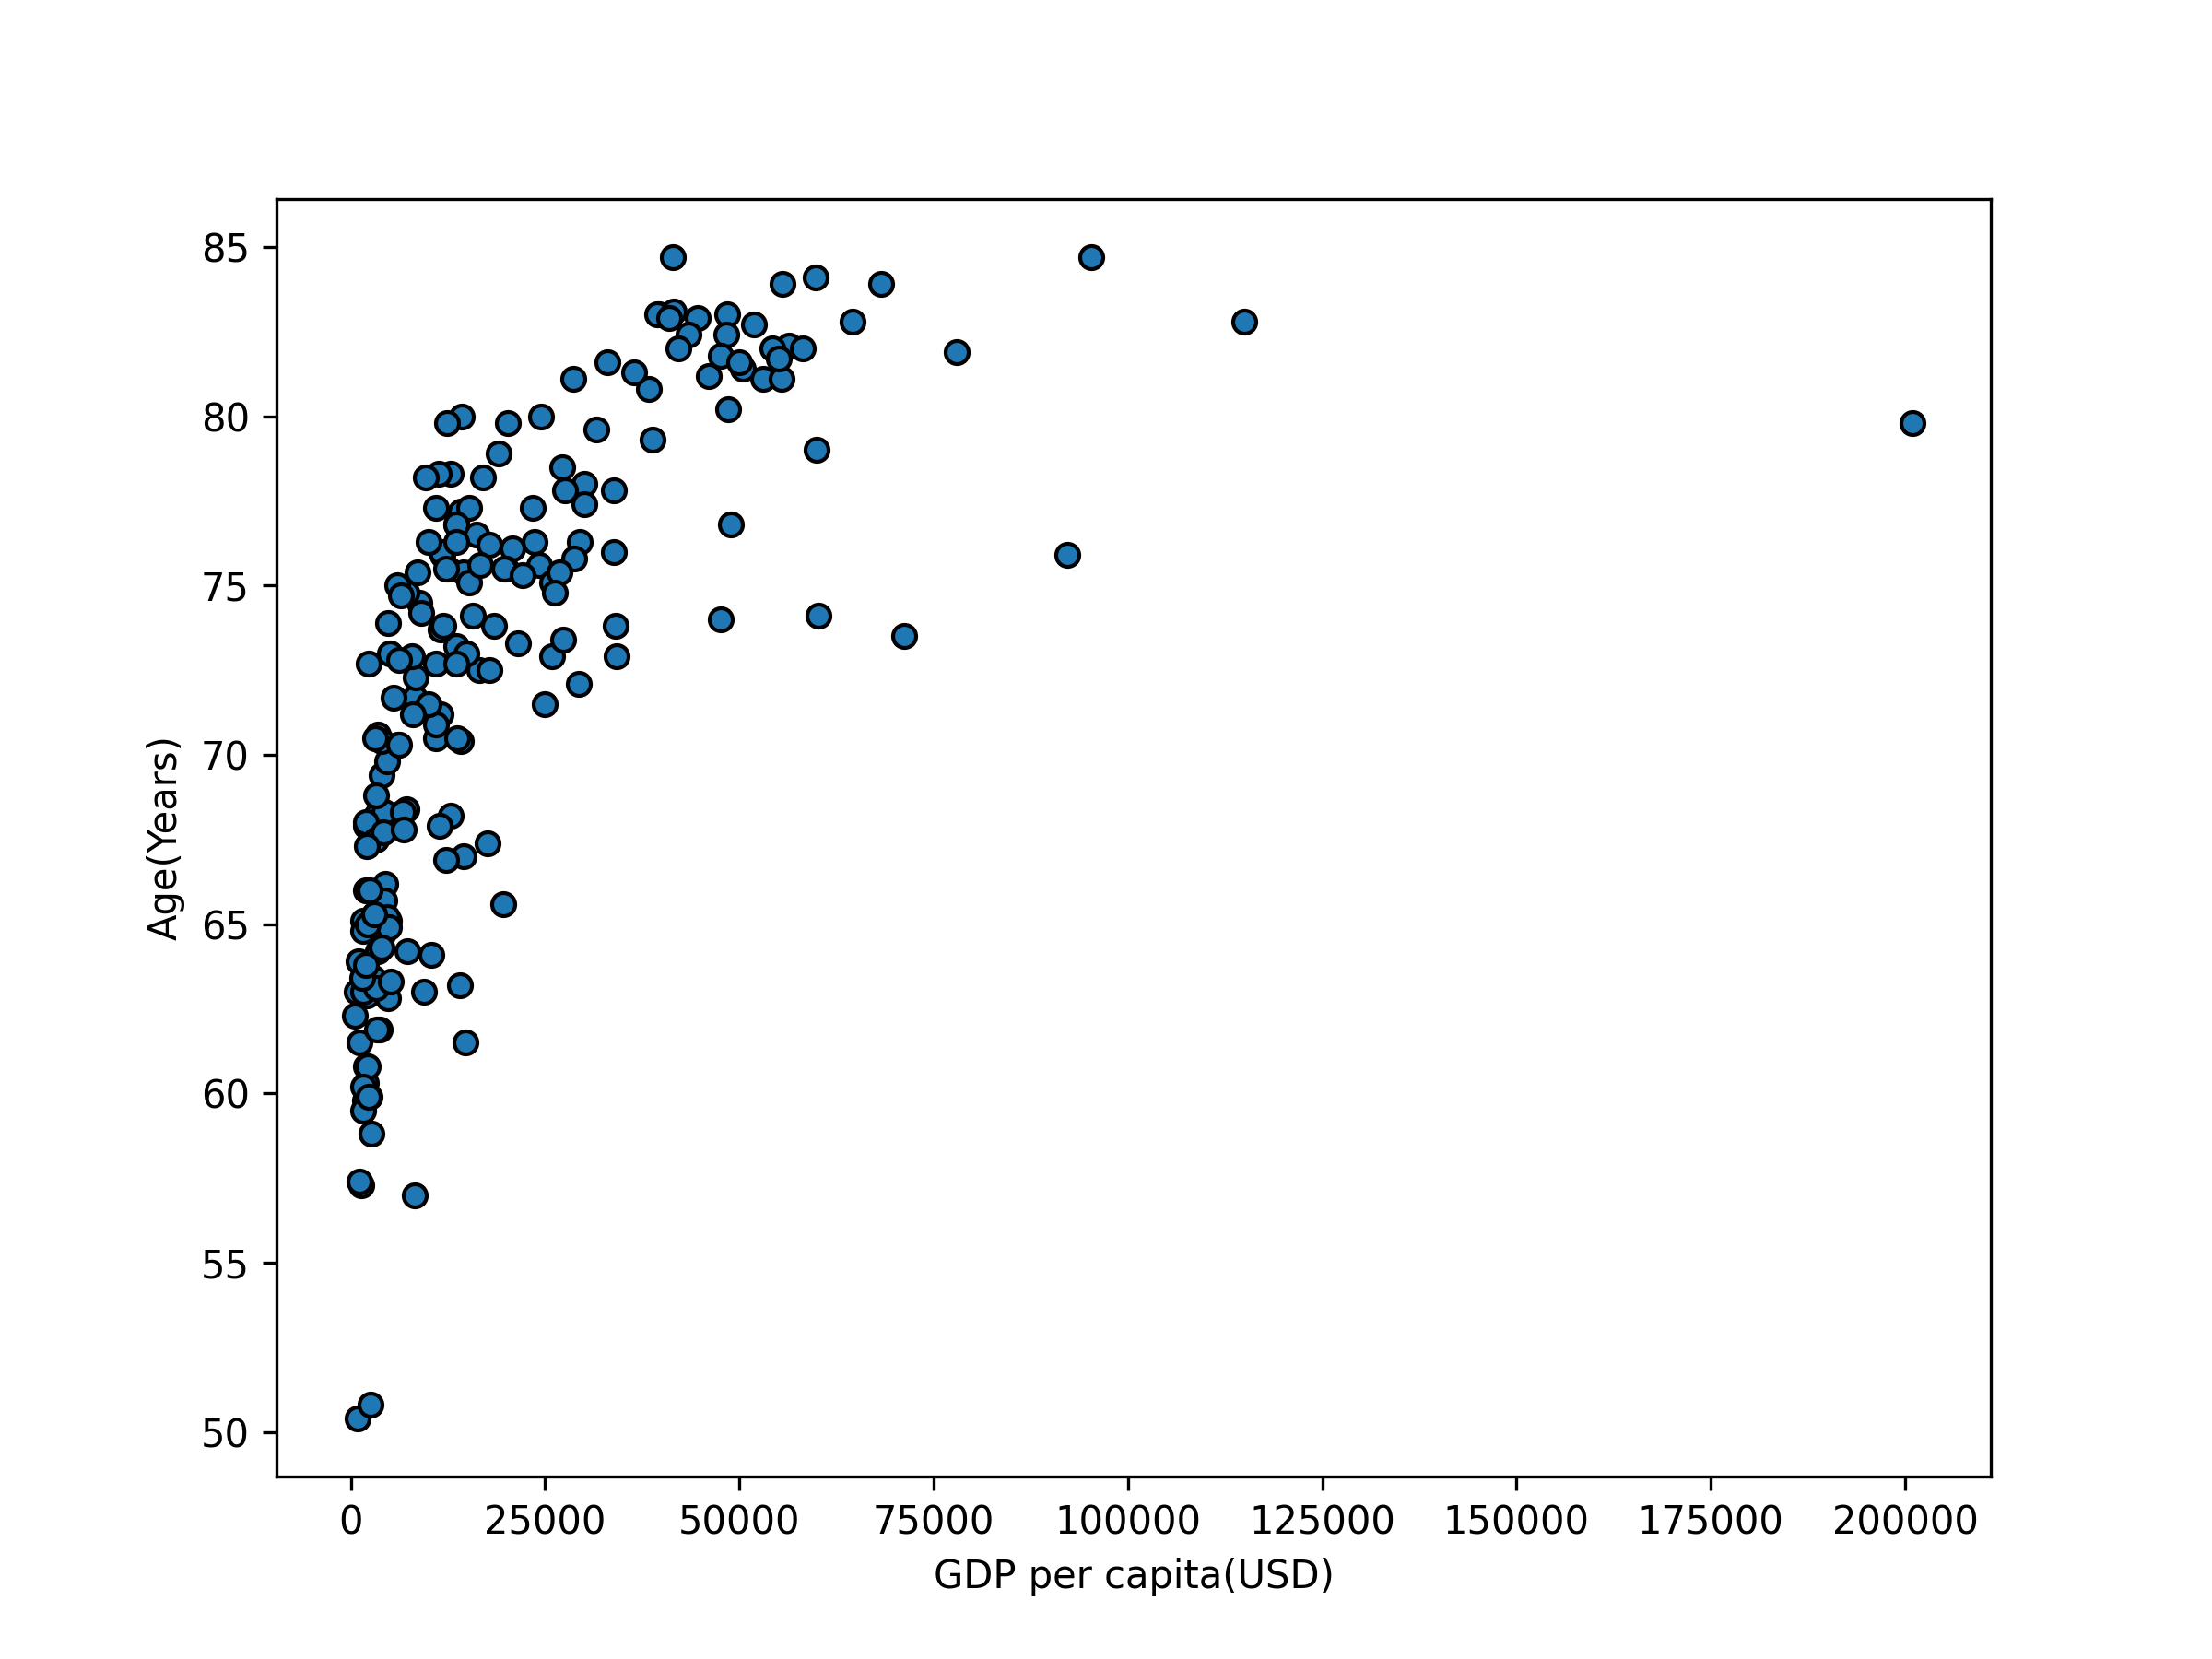
\includegraphics[width=0.8\textwidth]{figures/scatterplot.png}
    \caption{Correlation between GDP and Life Expectancy}
    \label{fig:gdp-lex-scatter}
\end{figure}
Since $r = 0.6402486572000062$, we can conclude that there's a moderate linear correlation between GDP and life span expectancy. However, a glance at the scatter plot tells us that there suggests a decelerating growth logarithmic correlation between the two fields. So we decided to check if the correlation between the natural logarithmic value of GDP and the life expectancy is stronger than the current one.

\begin{verbatim}
    correl2 = np.corrcoef(np.log(gdp), lex)[0, 1]
    print(correl2)
\end{verbatim}

And the result yields:
\begin{verbatim}
    0.8380396098306463
\end{verbatim}

It appears that a more robust linear correlation exists between the logarithmic values of GDP and life expectancy. Here's the visualization of the data.
\newpage
\begin{figure}[t]
    \centering
    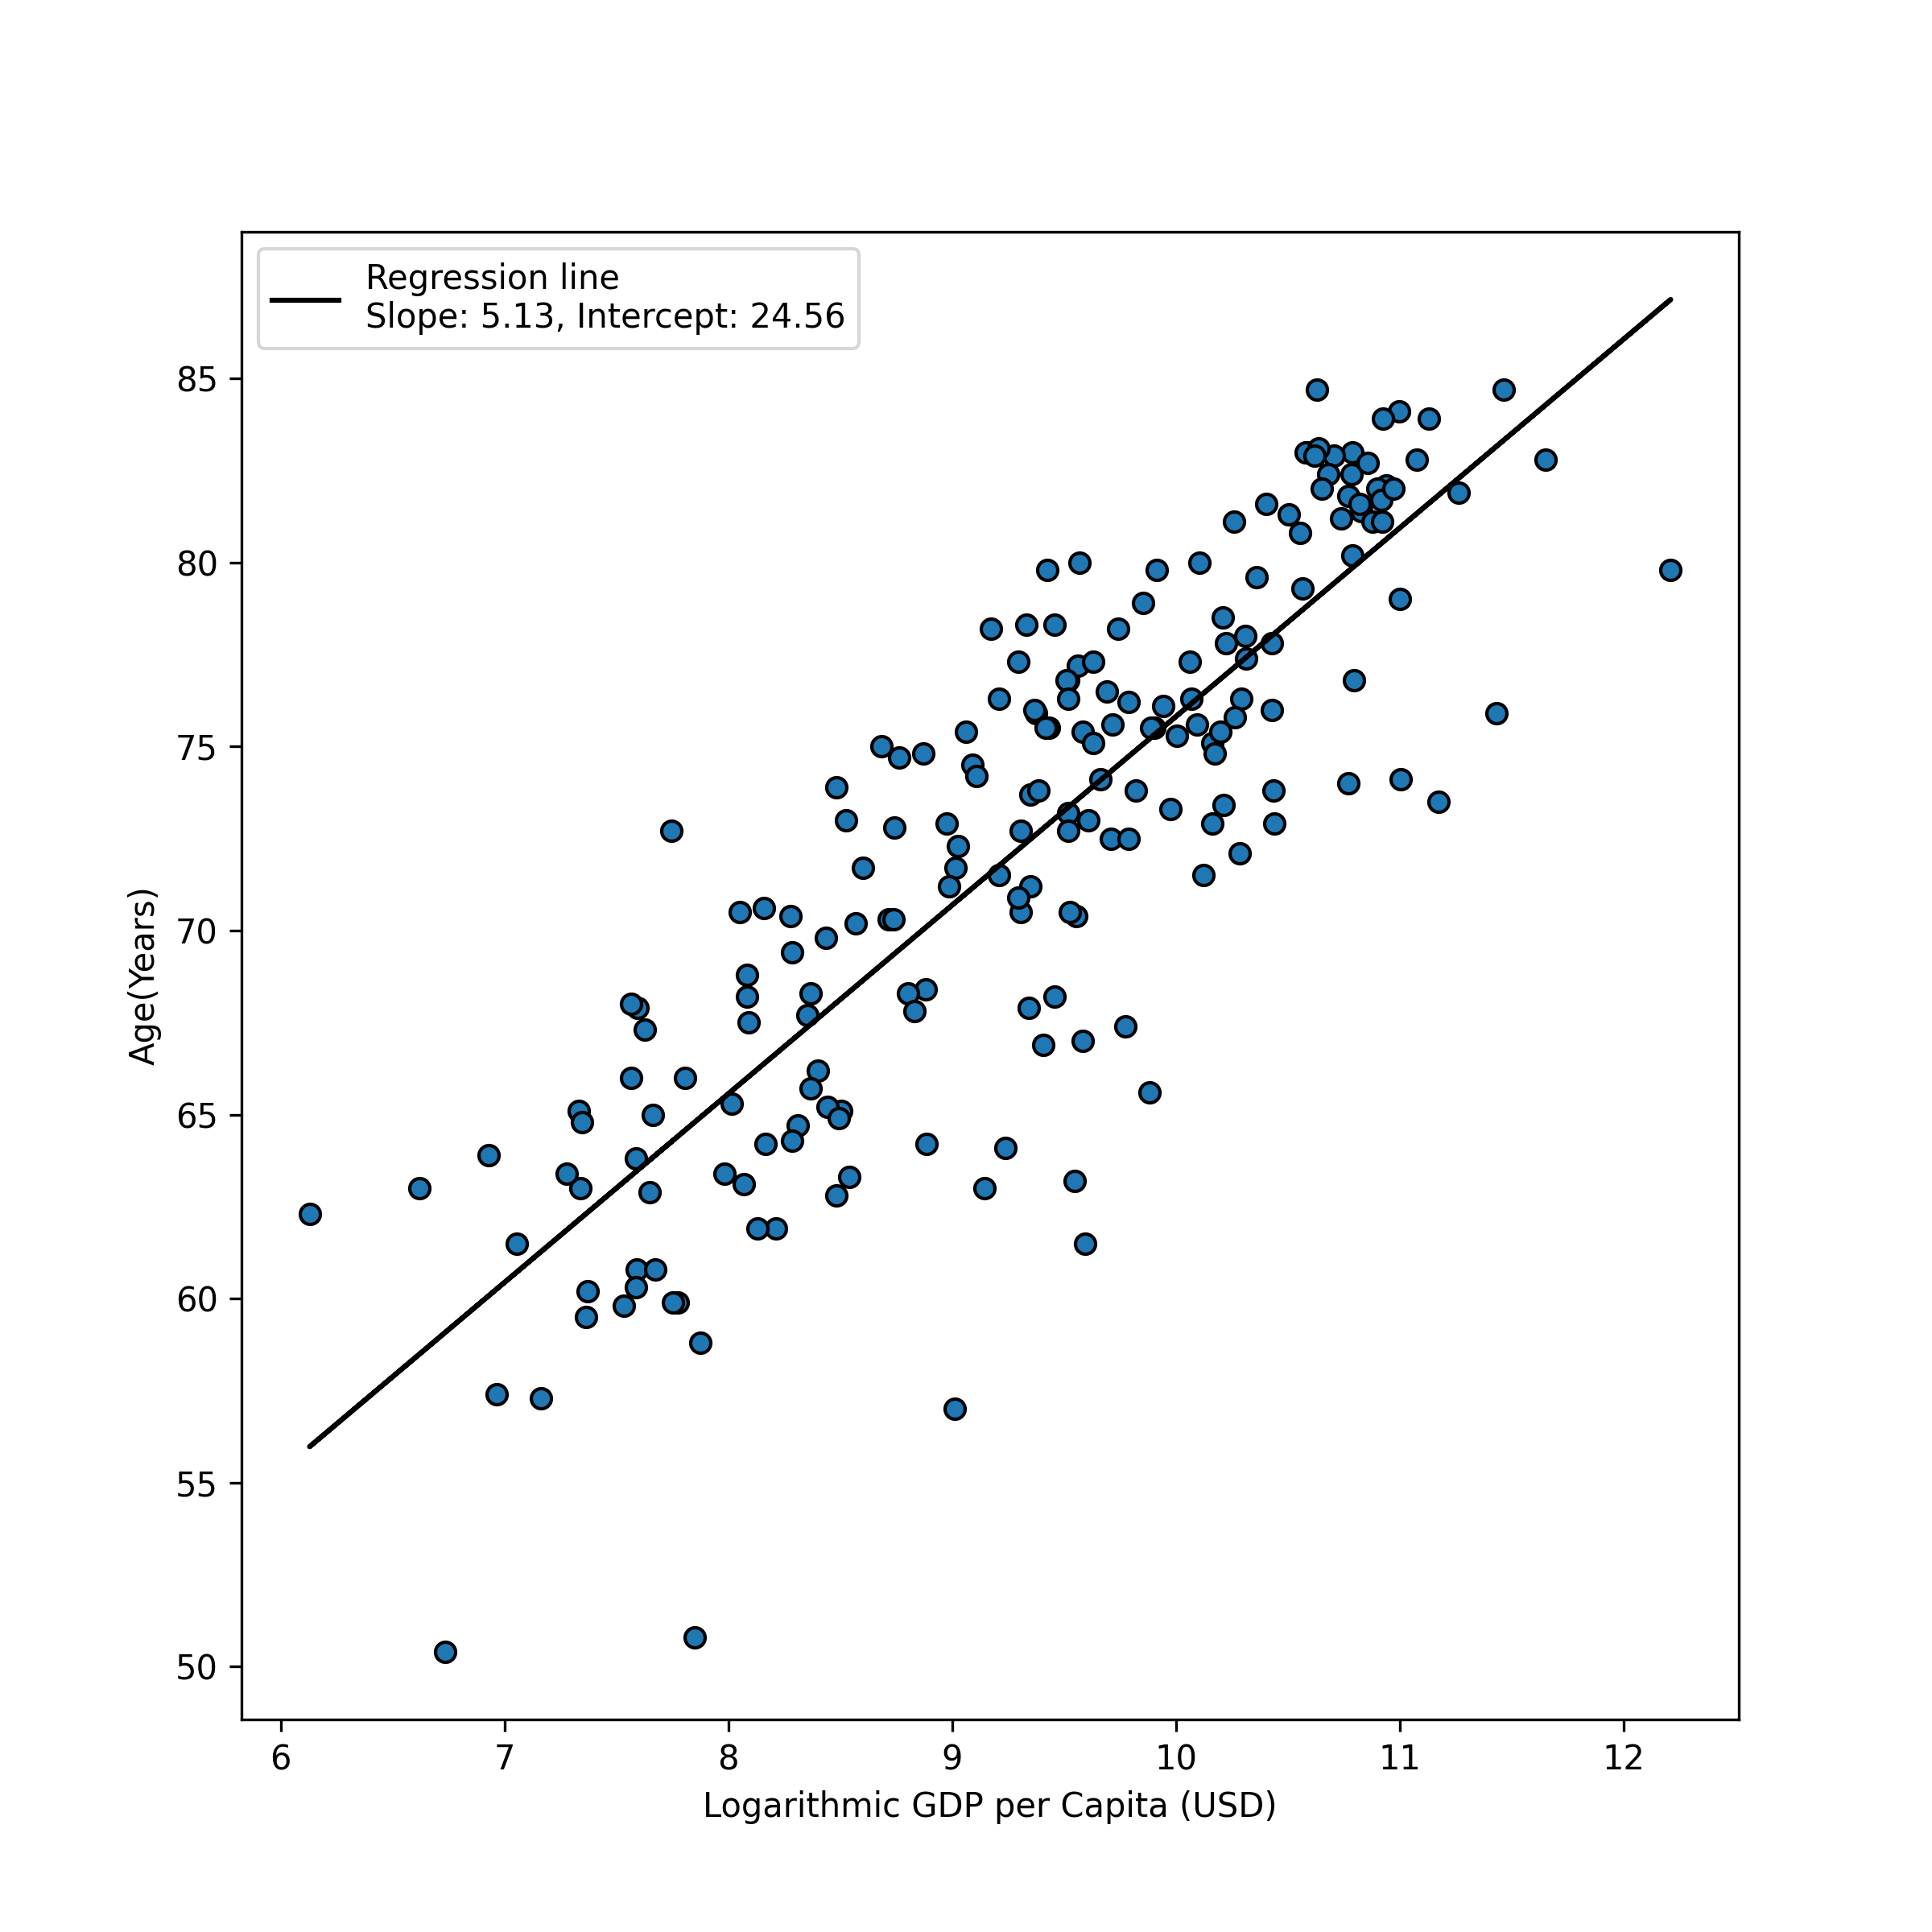
\includegraphics[width=0.8\textwidth]{figures/scatterplot2.png}
    \caption{Correlation between ln(GDP) and Life Expectancy}
    \label{fig:gdp-lex-scatter2}
\end{figure}

With these calculation, we can reasonably predict that a country with GDP of 100000 USD is expected to have a life expectancy of $slope * ln(GDP) + intercept = 5.13 * ln(100000) + 24.56 = 83.62$ (years)